\documentclass[12pt]{article}
 
\usepackage[margin=1in]{geometry} 
\usepackage{amsmath,amsfonts,amsthm,amssymb}
\usepackage{mathtools}
\usepackage{pifont}
\usepackage{graphics}
\usepackage{graphicx}
\usepackage{array}
\usepackage{listings}
\usepackage{matlab-prettifier}
\usepackage[hidelinks]{hyperref}
\usepackage{caption}
\usepackage{enumitem}

\lstdefinestyle{tex-style} {
	language=Matlab,                           % Code langugage
	basicstyle=\ttfamily,                   % Code font, Examples: \footnotesize, \ttfamily
	%keywordstyle=\color{OliveGreen},        % Keywords font ('*' = uppercase)
	commentstyle=\color{gray},              % Comments font
	numbers=none,                           % Line nums position
	numberstyle=\tiny,                      % Line-numbers fonts
	stepnumber=1,                           % Step between two line-numbers
	numbersep=5pt,                          % How far are line-numbers from code
	%backgroundcolor=\color{gray}, % Choose background color
	frame=single,                             % A frame around the code
	tabsize=2,                              % Default tab size
	captionpos=b,                           % Caption-position = bottom
	breaklines=true,                        % Automatic line breaking?
	breakatwhitespace=false,                % Automatic breaks only at whitespace?
	showspaces=false,                       % Dont make spaces visible
	showtabs=false,                         % Dont make tabls visible
	columns=flexible,                       % Column format
	morekeywords={__global__, __device__}  % CUDA specific keywords
}
\lstset{style=tex-style}
 
\newcommand{\N}{\mathbb{N}}
\newcommand{\Z}{\mathbb{Z}}
 
\newenvironment{theorem}[2][Theorem]{\begin{trivlist}
\item[\hskip \labelsep {\bfseries #1}\hskip \labelsep {\bfseries #2.}]}{\end{trivlist}}
\newenvironment{lemma}[2][Lemma]{\begin{trivlist}
\item[\hskip \labelsep {\bfseries #1}\hskip \labelsep {\bfseries #2.}]}{\end{trivlist}}
\newenvironment{exercise}[2][Exercise]{\begin{trivlist}
\item[\hskip \labelsep {\bfseries #1}\hskip \labelsep {\bfseries #2.}]}{\end{trivlist}}
\newenvironment{problem}[2][Problem]{\begin{trivlist}
\item[\hskip \labelsep {\bfseries #1}\hskip \labelsep {\bfseries #2.}]}{\end{trivlist}}
\newenvironment{question}[2][Question]{\begin{trivlist}
\item[\hskip \labelsep {\bfseries #1}\hskip \labelsep {\bfseries #2.}]}{\end{trivlist}}
\newenvironment{corollary}[2][Corollary]{\begin{trivlist}
\item[\hskip \labelsep {\bfseries #1}\hskip \labelsep {\bfseries #2.}]}{\end{trivlist}}

\newenvironment{solution}{\begin{proof}[Solution]}{\end{proof}}

%%%%%%% Table Packages %%%%%%%%%%%%%%%%%%%%%%%
\usepackage{booktabs}
\usepackage{multirow}
\usepackage{array}
\usepackage[T1]{fontenc}
\usepackage[utf8]{inputenc} 
\usepackage{tabularx,ragged2e,booktabs}
\newcolumntype{C}[1]{>{\Centering}m{#1}}
\renewcommand\tabularxcolumn[1]{C{#1}}
\newcommand{\ra}[1]{\renewcommand{\arraystretch}{#1}}
\usepackage{makecell}
\usepackage{tikz}
\usetikzlibrary{tikzmark,calc}
\usepackage{siunitx}
\usepackage[hidelinks]{hyperref}
\usepackage{amsmath}

 
\begin{document}
 
% --------------------------------------------------------------
%                         Start here
% --------------------------------------------------------------
 
\title{Homework 7}
\author{MEGN544/ROBO554 Robot Mechanics: Kinematics, Dynamics, and Control  
\\ 
Dr. George Kontoudis\\
Department of Mechanical Engineering\\
Colorado School of Mines}
\date{Fall 2026}
 
\maketitle
\begin{problem}{1}%theorem, exercise, problem, or question 
Calculate the time derivative of the following rotation matrices:
\begin{enumerate}[label=(\alph*)]
    \item $ \boldsymbol{\omega} = 
            \begin{bmatrix}
                0 \\ 0 \\ 1
            \end{bmatrix}\,\textrm{rad/s},~\boldsymbol{R} = 
            \begin{bmatrix}
                0.5 & -0.866 & 0 \\
                0.866 & 0.5 & 0 \\
                0 & 0 & 1
            \end{bmatrix}.$
    \item $ \boldsymbol{\omega} = 
            \begin{bmatrix}
                0 \\ 1 \\ 0
            \end{bmatrix}\,\textrm{rad/s},~\boldsymbol{R} = 
            \begin{bmatrix}
                0.5 & -0.866 & 0 \\
                0.866 & 0.5 & 0 \\
                0 & 0 & 1
            \end{bmatrix}.$
    \item $ \boldsymbol{\omega} = 
            \begin{bmatrix}
                1 \\ 0 \\ 0
            \end{bmatrix}\,\textrm{rad/s},~\boldsymbol{R} = 
            \begin{bmatrix}
                0.5 & -0.866 & 0 \\
                0.866 & 0.5 & 0 \\
                0 & 0 & 1
            \end{bmatrix}.$
    \item $ \boldsymbol{\omega} = 
            \begin{bmatrix}
                0.91340 \\ 0.63240 \\ 0.09754
            \end{bmatrix}\,\textrm{rad/s},~\boldsymbol{R} = 
            \begin{bmatrix}
                -0.62170 & -0.02073 & -0.78300 \\
                -0.13850 & -0.98100 & \ \ \, 0.13590 \\
                -0.77090 & \ \ \, 0.19300 & \ \ \, 0.60700
            \end{bmatrix}.$
\end{enumerate}
The angular velocity $ \boldsymbol{\omega}$ is expressed in the fixed frame. 
\end{problem}
%%%%%-------------------------------%%%%%%
\begin{problem}{2}%theorem, exercise, problem, or question 
A quadcopter is flying around with an inertial measurement unit (IMU) attached $10\,$cm offset from the center of mass (Figure~\ref{fig:drone}). An external observer measures the position, orientation, linear and angular velocity, and linear acceleration of the quadcopter relative to a fixed ground reference system (origin $0$). What is the linear velocity and acceleration, and angular velocity measured by the IMU in the body frame of the quadcopter at this instant? The angular velocity remains constant.
\textit{Hint: Do not forget gravity}.\\

\noindent $\prescript{0}{}{\boldsymbol{d}}_{01} = 
    \begin{bmatrix}
        20 \\ 15 \\ 10
    \end{bmatrix}\,\textrm{m},~
 \prescript{0}{}{\boldsymbol{R}}_{1} =
    \begin{bmatrix}
        0.5 & -0.866 & 0 \\
        0.866 & 0.5 & 0 \\
        0 & 0 & 1
    \end{bmatrix},~
 \prescript{0}{}{\boldsymbol{v}}_{01} = 
    \begin{bmatrix}
        10 \\ 5 \\ 0.25
    \end{bmatrix}\,\textrm{m/s},~   
 \prescript{0}{}{\boldsymbol{a}}_{01} = 
    \begin{bmatrix}
        -1 \\ 0 \\ 0.1
    \end{bmatrix}\,\textrm{m/s}^2, \\
 \prescript{0}{}{\boldsymbol{\omega}}_{01} = 
    \begin{bmatrix}
        0 \\ 0 \\ 2.3
    \end{bmatrix}\,\textrm{rad/s}$.

    \begin{figure}[!h]
	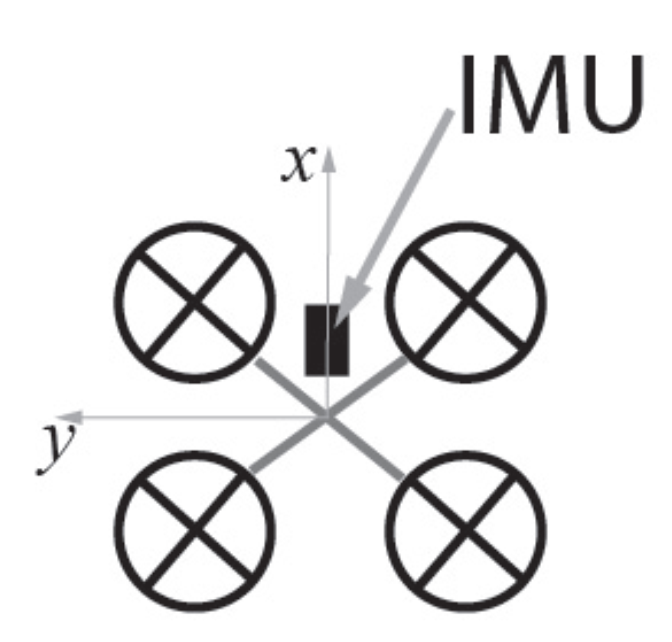
\includegraphics[width=.25\columnwidth]{figures/drone_imu.png}
	\centering
	\caption{IMU offset from the center of mass.}
	\label{fig:drone}
\end{figure}

\end{problem}
\newpage
%%%%%-------------------------------%%%%%%
\begin{problem}{3}%theorem, exercise, problem, or question 
Consider a three-link manipulator with joint angles $\boldsymbol{\theta} = [\pi/3 \ \ \pi/6 \ \ \pi/6]^{\intercal}$ rad, joint angle rates $\dot{\boldsymbol{\theta}} = [0.5 \ \ -1.0\ \ 1.5]^{\intercal}$~rad/s, a stationary base, and the following DH table.  Assume that the angle rates remain constant. What are the angular velocities $\boldsymbol{\omega}_i$, linear velocities $\dot{\boldsymbol{d}}_{0,i}$, and accelerations $\ddot{\boldsymbol{d}}_{0,i}$ at each frame (i.e., $i=1,2,3$)? In addition, construct the velocity Jacobian. \textit{Hint: The velocity of the end frame is } $\boldsymbol{J}_{\textrm{v}} \dot{\boldsymbol{\theta}} = [ -0.1924\ \ 0.2498\ \ {-0.3580}\ \ 0.4330\ \ -0.2500\ \ 0.5000]^{\intercal}$.

\begin{table}[!h]
\centering
\begin{tabular}{c | c | c | c | c}
\hline 
 {Link} & $a$   & $d$  & $\alpha$ & $\theta$\\  \hline
 $1$    & $0$   & $1$  & $\pi/2$  & $\star$ \\ 
 $2$    & $0.5$ & $0$  & $0$      & $\star$ \\ 
 $3$    & $0.3$ & $0$  & $0$      & $\star$ \\  \hline
\end{tabular}\label{tab:part_1_ii}
\end{table}


\end{problem}

\end{document}